\documentclass[12pt,letterpaper]{article}
\usepackage[latin1]{inputenc}
\usepackage[spanish]{babel}
\usepackage{graphicx}
\usepackage[left=2cm,right=2cm,top=2cm,bottom=2cm]{geometry}
\usepackage{graphicx} % figuras
\usepackage{subfigure} % subfiguras
\usepackage{float} % para usar [H]
\usepackage{amsmath}
\usepackage{txfonts}
\usepackage{stackrel} 
\usepackage[latin1]{inputenc}
\usepackage{multirow}
\usepackage{enumerate} % enumerados
\renewcommand{\labelitemi}{$-$}
\renewcommand{\labelitemii}{$\cdot$}

\begin{document}


\begin{titlepage}
\begin{center}
\large{UNIVERSIDAD PRIVADA DE TACNA}\\
\vspace*{-0.025in}
\begin{figure}[htb]
\begin{center}

\includegraphics[width=8cm]{./IMG/logo}
\end{center}
\end{figure}
\vspace*{0.15in}
INGENIERIA DE SISTEMAS  \\

\vspace*{0.5in}
\begin{large}
TITULO:\\
\end{large}

\vspace*{0.1in}
\begin{Large}
\textbf{PRACTICA DE LABORATORIO Nro 05} \\
\end{Large}

\vspace*{0.3in}
\begin{Large}
\textbf{CURSO:} \\
\end{Large}

\vspace*{0.1in}
\begin{large}
INTELIGENCIA DE NEGOCIOS\\
\end{large}

\vspace*{0.3in}
\begin{Large}
\textbf{DOCENTE:} \\
\end{Large}

\vspace*{0.1in}
\begin{large}
 Ing. Patrick Cuadros\\
\end{large}

\vspace*{0.2in}
\vspace*{0.1in}
\begin{large}
ESTUDIANTE: \\
\begin{flushleft}

Villegas Arando, Marlon Xavier 		\hfill	(2015053890) \\

\end{flushleft}
\end{large}
\end{center}

\end{titlepage}

 \newpage

\section{Desarrollo} 
I.	INFORMACION GENERAL\\

1.	OBJETIVO GENERAL\\
Proveer soporte para actividades de toma de decision basado en informacion empirica El objetivo principal vendria a ser la creacion de una Data Warehouse esta data base nos va a permitir disminuir la data base original siendo mas facil y accesible para una creacion de inteligencia de negocios, tambien vamos a crear nuestro Data Source, Data Flow con sus diferentes Queries de cada Dimension\\

2.	OBJETIVO ESPECIFICO\\
Desarrollar los siguientes puntos para este trabajo de la segunda unidad:\\

- Arquitectura de BI para su Empresa\\
- Dise\~no Dimensional L\'ogico y Fisico\\
- Detallar los Procesos de Negocios de su trabajo\\
- Requerimientos de Negocios\\
- Identificar las Dimensiones\\
- Identificar las Jerarqu\'ias\\
- Identificar los Hechos\\
- Identificar las M\'etricas\\
- Realizar el Modelado\\
- Crear el DW en un SGBD como SQL Server\\
- Desarrollo de ETL\\
- An\'alisis de los Datos\\
- Mapeo (Realizar un mapeo entre DW y Data Source)\\
- Conexiones a Base de Datos (Detallar las conexiones a datos)\\
- Desarrollo de DTSX (DataFlow, Queries)\\

II.	DESARROLLO DEL PROYECTO(VIM)

1.	ARQUITECTURA DE BI PARA SU EMPRESA

\begin{center}
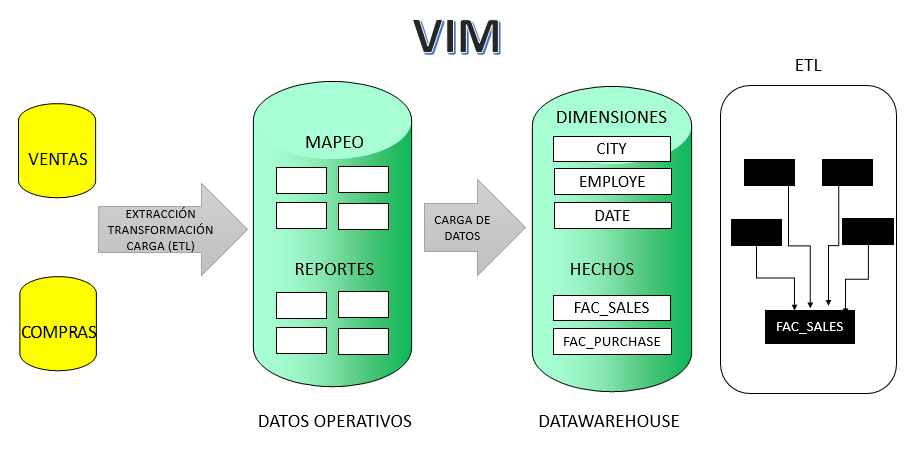
\includegraphics[width=17cm]{IMG/empresa.png} 
\end{center}

2. Restaurar Backup Workstationa2012

\begin{center}
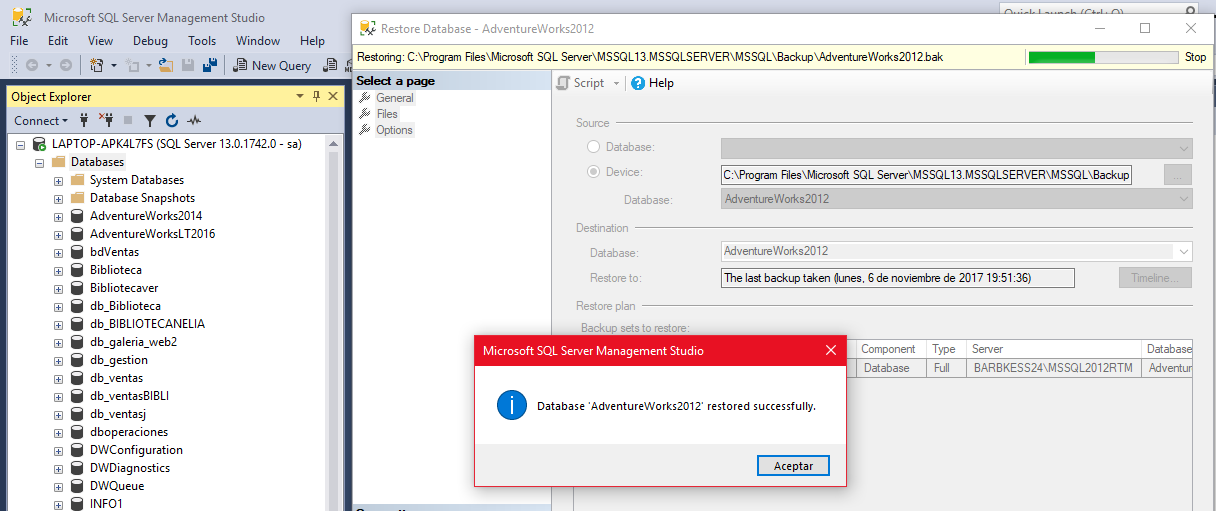
\includegraphics[width=17cm]{IMG/backup.png} 
\end{center}

II.	DESARROLLO DIMENSIONAL LOGICO Y FISICO
- DISE\~NO LOGICO
- Proceso de Ventas

\begin{center}
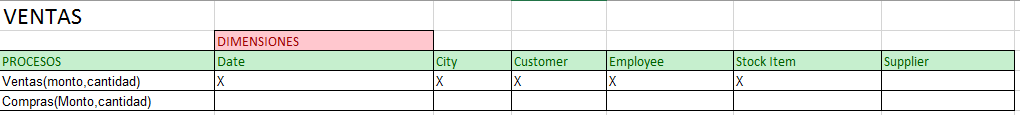
\includegraphics[width=17cm]{IMG/3.png} 
\end{center}
 \newpage

\begin{center}
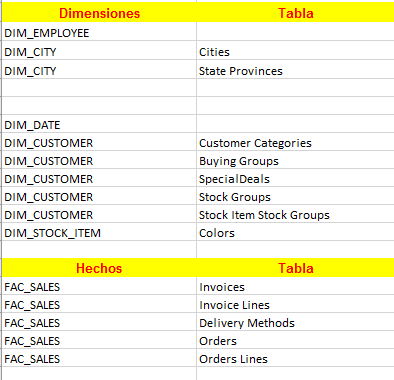
\includegraphics[width=15cm]{IMG/4.png} 
\end{center}
\begin{center}
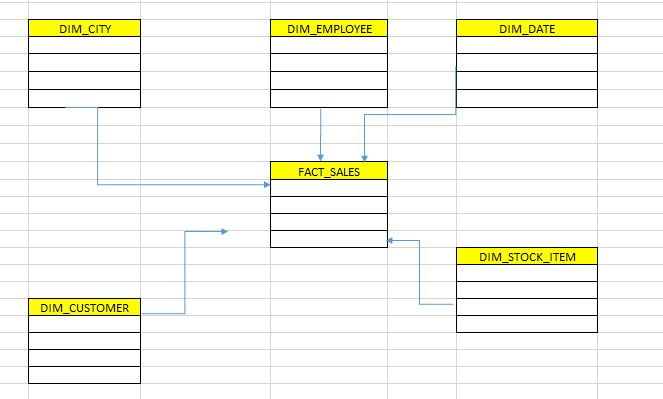
\includegraphics[width=15cm]{IMG/5.png} 
\end{center}

- Proceso de Ventas

\begin{center}
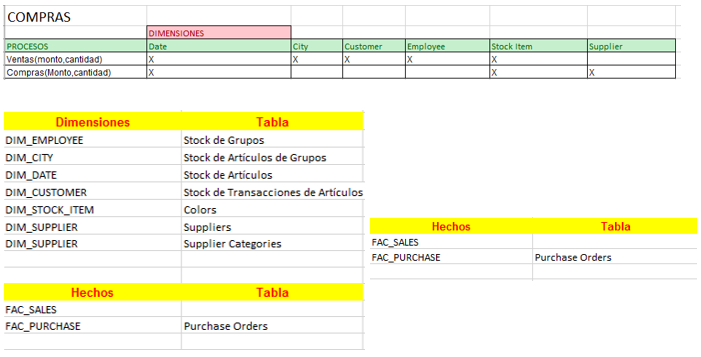
\includegraphics[width=17cm]{IMG/6.png} 
\end{center}

\begin{center}
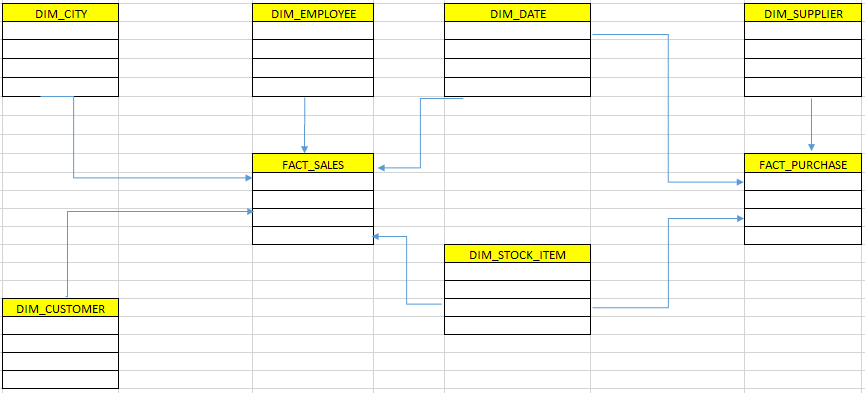
\includegraphics[width=17cm]{IMG/7.png} 
\end{center}

- Dise\~no Fisico

\begin{center}
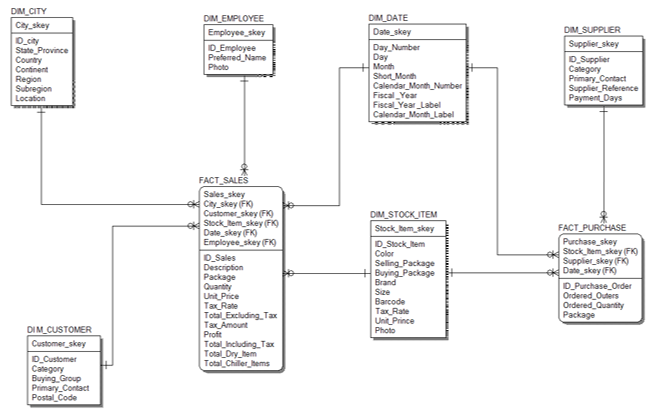
\includegraphics[width=17cm]{IMG/8.png} 
\end{center}

A.	DETALLAR LOS PROCESOS DE NEGOCIOS DE SU TRABAJO\\

Lo que vamos a conocer en nuestro trabajo, del proyecto que vamos a presentar tenemos asignados a dos procesos, que va a ser ventas y compras, tambi\'en tenemos en total 6 dimensiones, el primer proceso va a ser Ventas va a tener las siguientes dimensiones, Date, City, Customer, Employee, Stock Item, y el segundo proceso va a ser Compras va tener las siguientes dimensiones, Date Stock Item, y Supplier.

\begin{center}
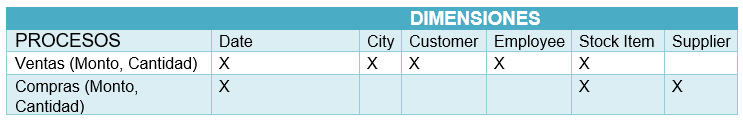
\includegraphics[width=17cm]{IMG/9.png} 
\end{center}

B.	REQUERIMIENTOS DE NEGOCIOS \\

Para nuestra empresa VIM tenemos algunos requerimientos que queremos tener en cuenta.\\

REQUERIMIENTOS GEN\'ERICOS\\
- proveer un sistema intuitivo y f\'acil de usar que permita a los usuarios finales generar sus propios reportes y an\'alisis.\\
- tener una sola versi\'on de la informaci\'on.\\
- proveer informaci\'on de toda la compa~n\'ia en un solo sistemas.\\
- que los usuarios puedan acceso la informaci\'on desde cualquier lugar y en cualquier momento.\\

REQUERIMIENTOS FUNCIONALES\\
- El sistema deber\'a tener los mecanismos para controlar la seguridad de los datos por departamento, \'area, gerencia, as\'i como una distribucin organizacional jer\'arquica de la informaci\'on.\\
- el sistema proveer\'a un mecanismo de notificaciones y alertas, con criterios y reglas configurables.\\
- el sistema permitir\'a la integraci\'on de diferentes fuentes de datos.\\
- el sistema debe ser intuitivo para que los usuarios finales puedan desarrollar sus propios reportes.\\

REQUERIMIENTOS DE NEGOCIO\\
- Definir la estrategia de negocio en procesos que sean medibles y controlables.\\
- Identificar la informaci\'on necesaria para cada proceso de negocio, detallando su forma de an\'alisis, seguimiento, t\'ecnicas de an\'alisis y predicci\'on (s\'i aplica), as\'i como requerimientos tecnol\'ogicos para su cumplimiento.\\
- Priorizar los objetivos de la soluci\'on en funci\'on de su impacto en las metas del negocio.\\
- Dise\~nar una administraci\'on flexible que permita la adaptaci\'on de las estrategias del negocio a corto y mediano plazo basado en el aprendizaje continuo de la operaci\'on y seguimiento del negocio.\\

C.	IDENTIFICAR LAS DIMENSIONES\\
Ahora vamos a identificar las dimensiones de nuestros dos procesos de est\'a forma en la cu\'al estamos viendo de Ventas y Compras, de las dos tenemos 6 en total 5 son para Ventas y 3 son para Compras, pero dos de las dimensiones de Ventas se unen a nuestro Hecho Compras\\

\begin{center}
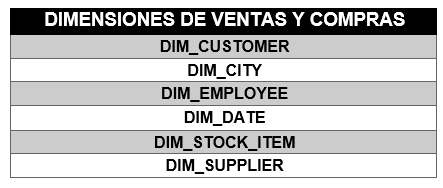
\includegraphics[width=17cm]{IMG/10.png} 
\end{center}

D.	IDENTIFICAR LAS JERARQUIAS\\

Se crearon jerarqu\'ias para las dimensiones de:\\

- CUSTOMER (Cliente)\\

Esta tiene el siguiente esquema:\\
- Grupo de Compra\\
- Categor\'ia\\
- Cliente\\

- CITY (Ciudad)\\

Esta tiene el siguiente esquema:\\
- Continente\\
- Pa\'is\\
- Ciudad\\

- EMPLOYEE (Empleado)\\

Esta tiene el siguiente esquema:\\
- Grupo de Venta\\
- Categor\'ia\\
- Employee\\



- DATE (Tiempo)\\

Esta tiene el siguiente esquema:\\
- A\~no\\
- Mes\\
- D\'ia\\

- STOCK ITEM (Producto)\\

Esta tiene el siguiente esquema:\\
- Marca\\
- Producto\\
- Color\\

- SUPPLIER (Proveedor)\\

Esta tiene el siguiente esquema:\\
- Grupo de Compra\\
- Categor\'ia\\
- Proveedor\\

E.	IDENTIFICAR LOS HECHOS\\

Aqu\'i tenemos nuestros Hechos con sus respectivas dimensiones dentro de cada Hecho, una tiene 5 que es FACTSALES este es el de ventas y el otro FACPURCHASE solo tiene dos una diferente y dos de la misma tabla de hechos de FACSALES que se unen a nuestro otro hecho\\
\begin{center}
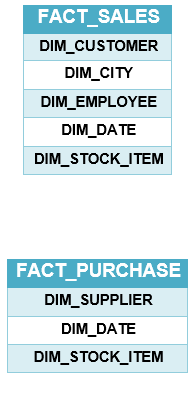
\includegraphics[width=5cm]{IMG/11.png} 
\end{center}

A.	IDENTIFICAR LAS METRICAS\\
Las m\'etricas que tiene nuestra empresa \\


\begin{center}
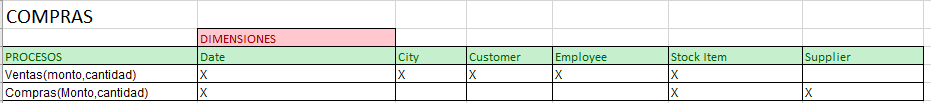
\includegraphics[width=17cm]{IMG/12.png} 
\end{center}

\begin{center}
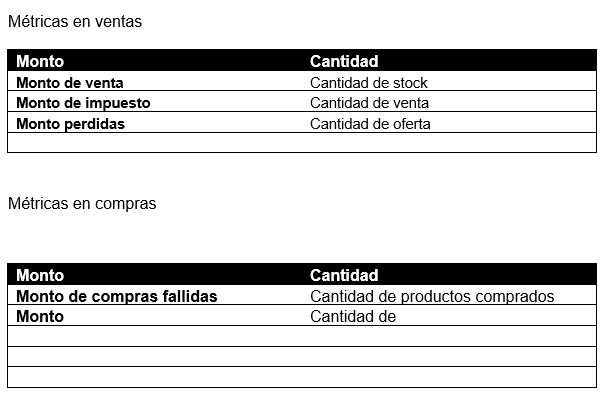
\includegraphics[width=17cm]{IMG/13.png} 
\end{center}

G.	REALIZAR EL MODELADO\\

Para realizar el modelado de dimensiones y hecho primero se hizo un an\'alisis de la base de datos transaccional luego pasamos seleccionar las tabas que vamos a utilizar para a realizaci\'on de la data warehouse.
Las tablas son las siguientes: \\

\begin{center}
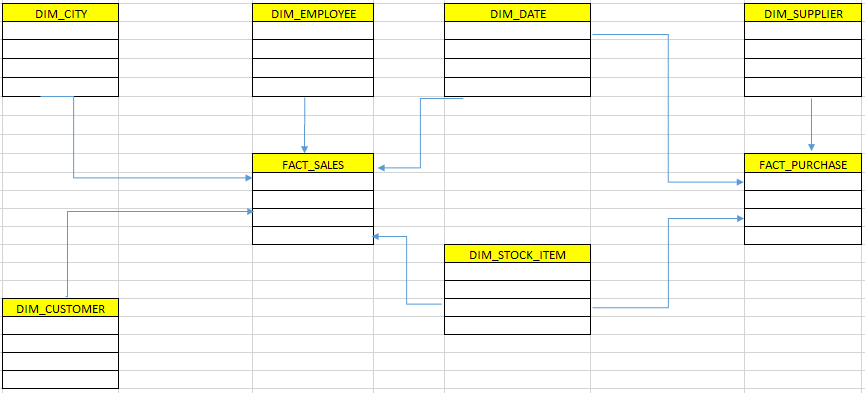
\includegraphics[width=17cm]{IMG/14.png} 
\end{center}

A.	CREAR EL DW EN UN SGBD COMO SQL SERVER\\

Para la realizaci\'on de nuestra data warehouse utilizamos el software  de sql server. \\

\begin{center}
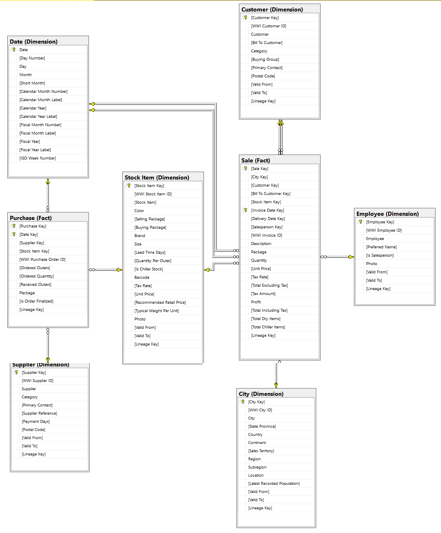
\includegraphics[width=17cm]{IMG/15.png} 
\end{center}

3.	DESARROLLO DE ETL\\

A.	ANALISIS DE LOS DATOS (DETALLAR)\\
Para la realizaci\'on de datos se hizo los siguientes query para cada dimencion y hechos.\\

\begin{center}
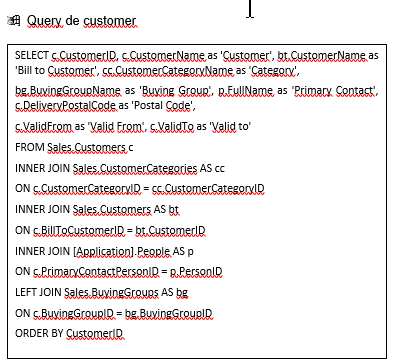
\includegraphics[width=17cm]{IMG/16.png} 
\end{center}

\begin{center}
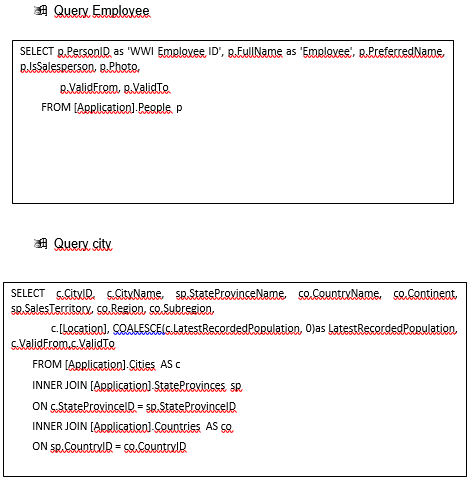
\includegraphics[width=17cm]{IMG/17.png} 
\end{center}

\begin{center}
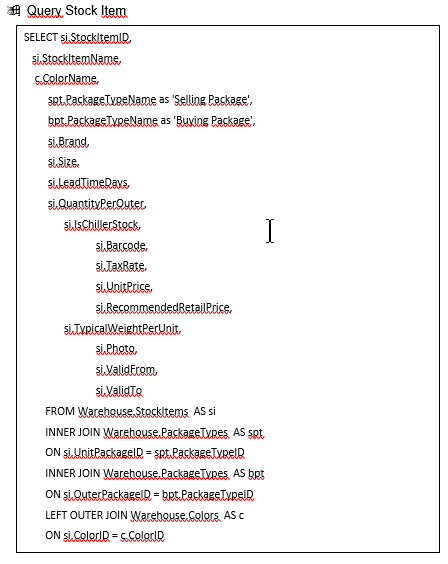
\includegraphics[width=17cm]{IMG/18.png} 
\end{center}

\begin{center}
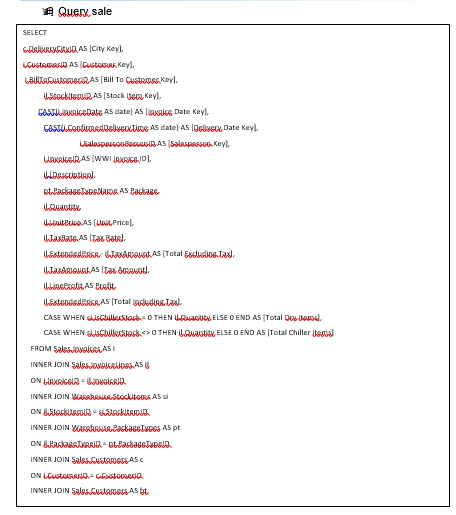
\includegraphics[width=17cm]{IMG/19.png} 
\end{center}

B.	MAPEO (REALIZAR UN MAPEO ENTRE DW Y DATA SOURCE) \\
Comenzamos el mapeo que esta contiene cada datos que tiene una tabla par ello vamos a colocar cada tabla para ver los datos.\\

- FAC-PURCHASE\\

\begin{center}
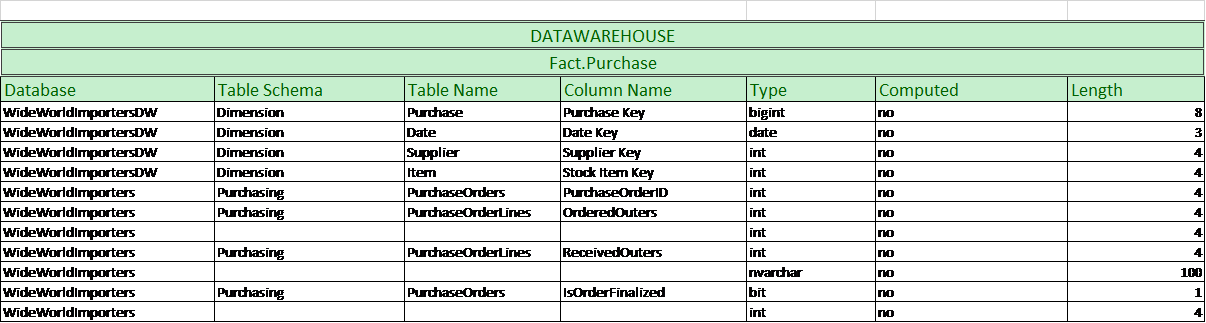
\includegraphics[width=17cm]{IMG/20.png} 
\end{center}
- DIM-stock-Item\\

\begin{center}
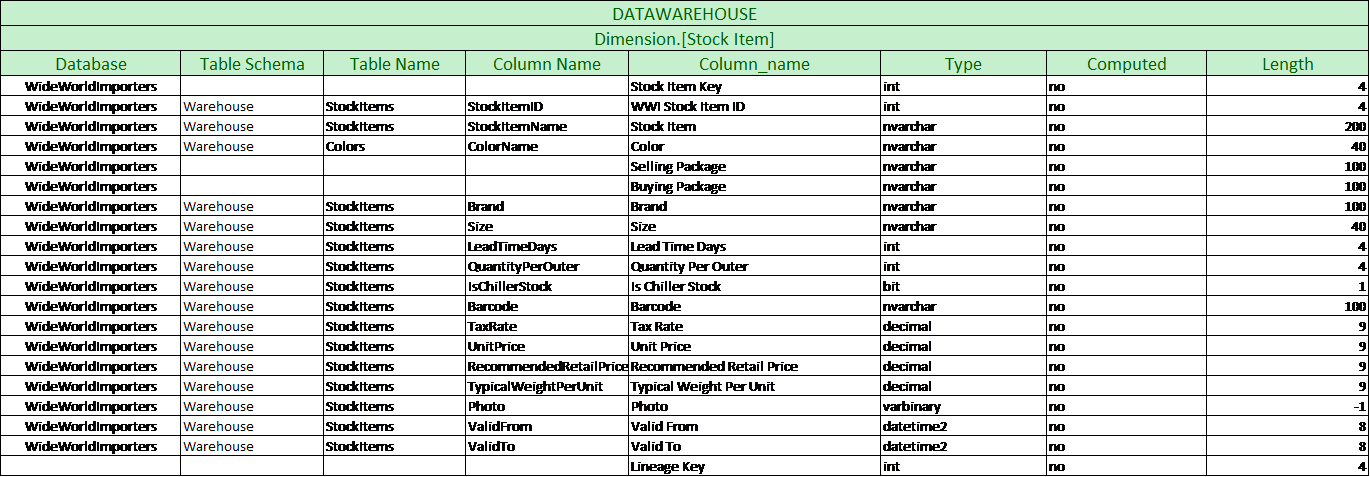
\includegraphics[width=17cm]{IMG/21.png} 
\end{center}

- DIM-Supplier\\

\begin{center}
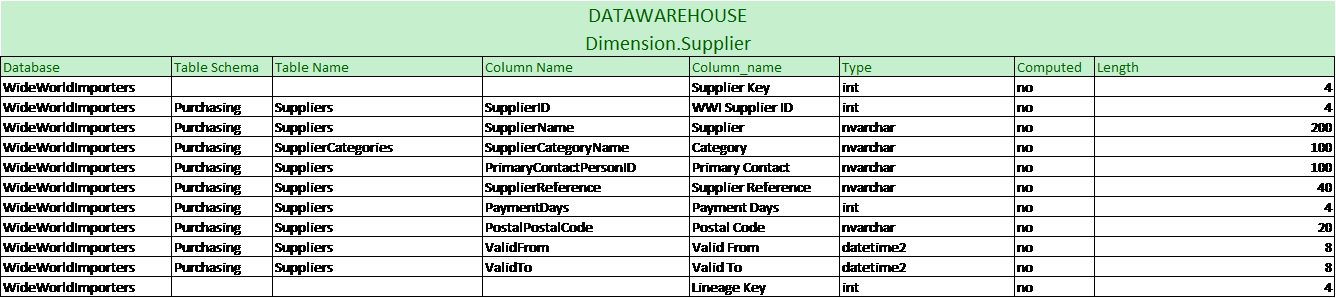
\includegraphics[width=17cm]{IMG/22.png} 
\end{center}

- FAC-SALES\\

\begin{center}
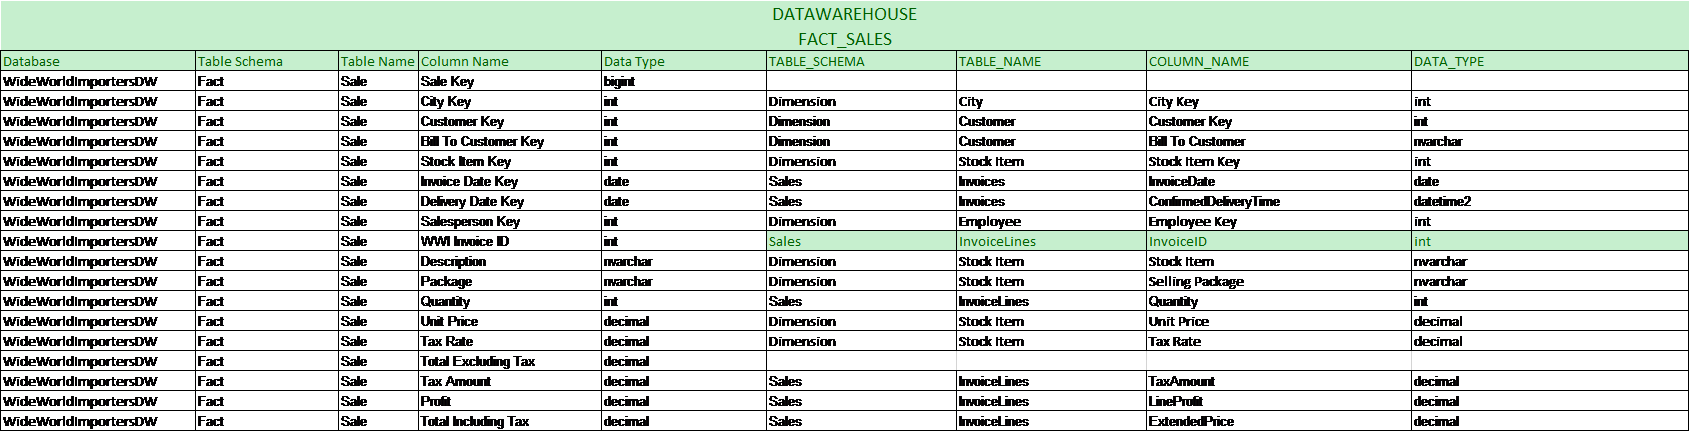
\includegraphics[width=17cm]{IMG/23.png} 
\end{center}
- DIM-CITY\\

\begin{center}
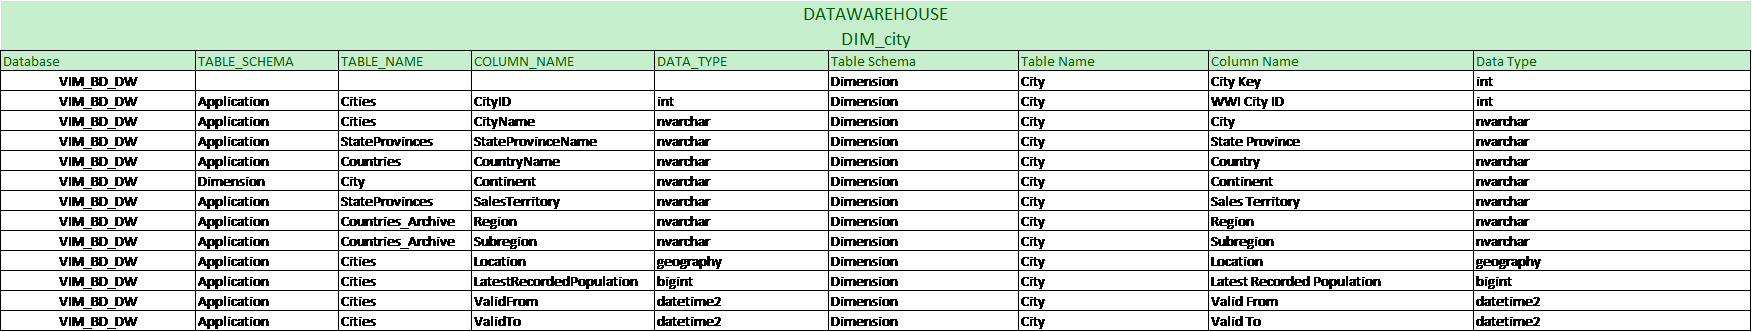
\includegraphics[width=17cm]{IMG/24.png} 
\end{center}

- DIM-EMPLOYE\\

\begin{center}
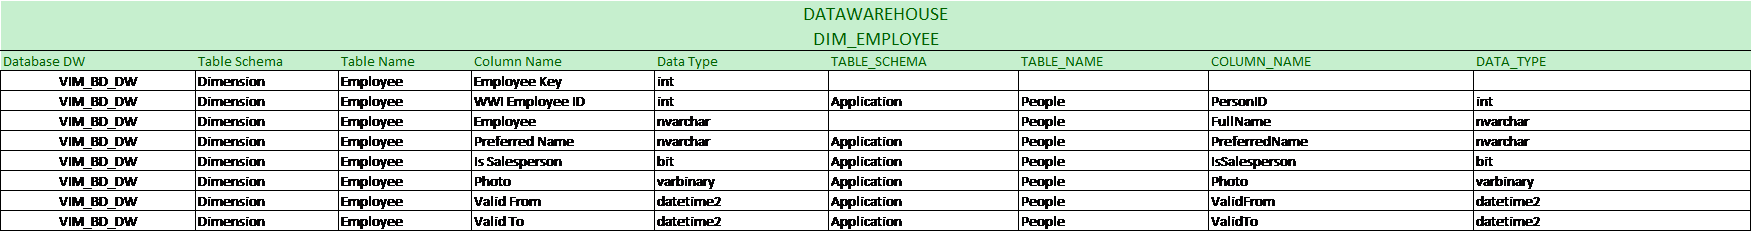
\includegraphics[width=17cm]{IMG/25.png} 
\end{center}

- DIM-CUSTOMER\\
\begin{center}
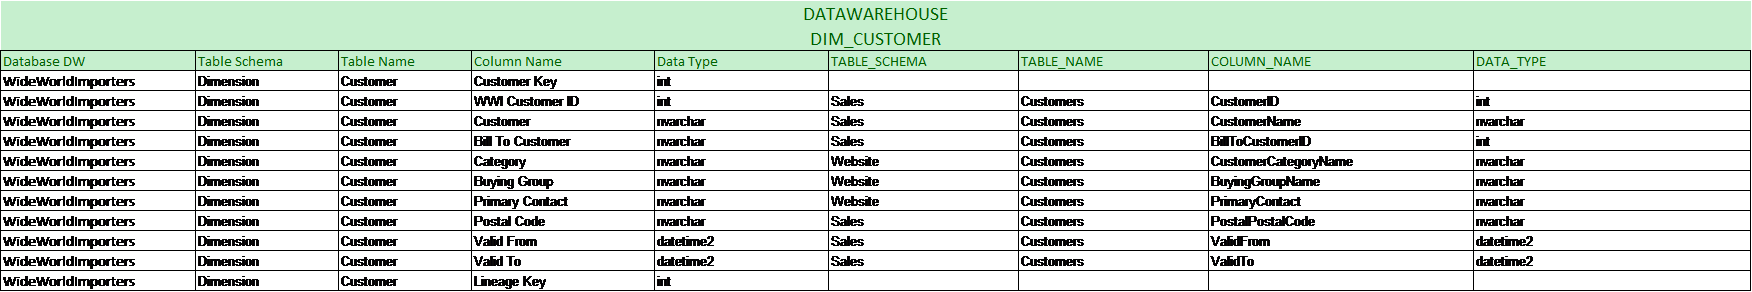
\includegraphics[width=17cm]{IMG/26.png} 
\end{center}

C.	CONECCIONES A BASE DE DATOS (DETALLAR LAS CONECCIONES A DATOS)\\


Ahora vamos a crear la conexi\'on de nuestra base de datos en nuestro programa de Data Flow, ponemos clic derecho y luego nueva conexi\'on\\
\begin{center}
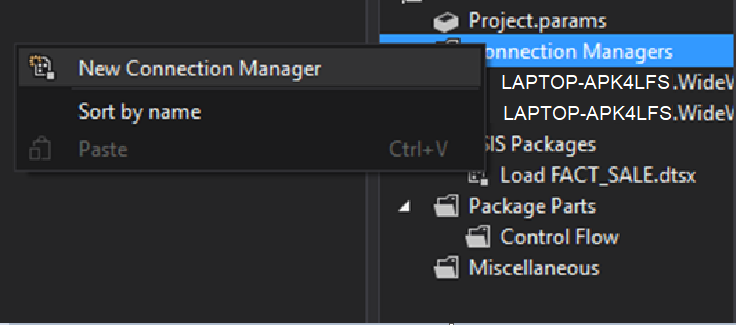
\includegraphics[width=9cm]{IMG/27.png} 
\end{center}

Ahora nos pide conectar el tipo de conexi\'on qu\'e vamos a tener, y nosotros trabajos con OLEDB y luego le damos clic en ADD agregar\\
\begin{center}
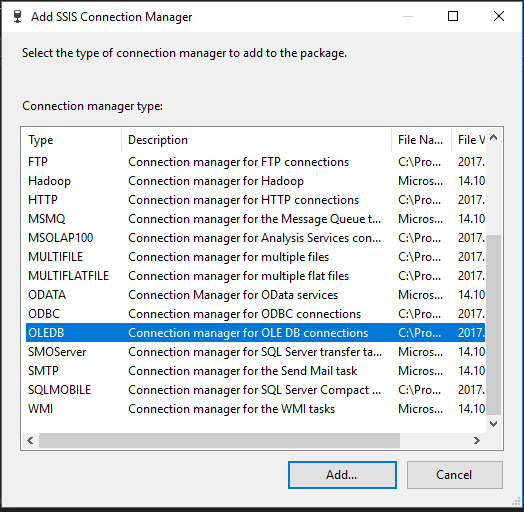
\includegraphics[width=17cm]{IMG/28.png} 
\end{center}

Luego vamos a poner el nombre de nuestra m\'aquina, que sería LAPTOP-APK4LFS, y lo ponemos\\

\begin{center}
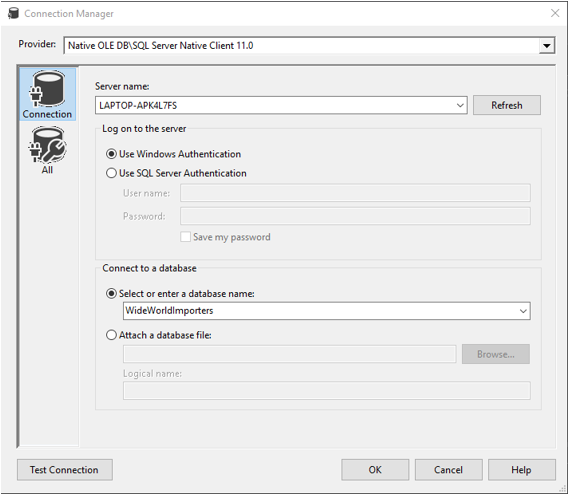
\includegraphics[width=17cm]{IMG/29.png} 
\end{center}
Luego escogemos nuestra base de datos transaccional y le damos clic en OK\\
\begin{center}
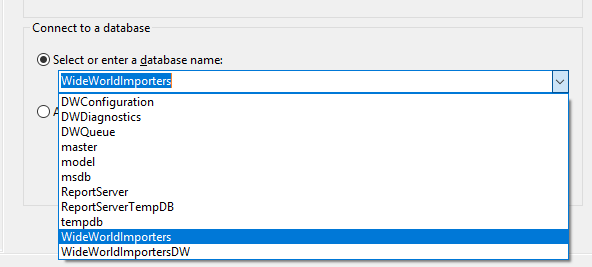
\includegraphics[width=17cm]{IMG/30.png} 
\end{center}
Luego vamos a crear otra nueva conexi\'on, y luego ponemos el nombre de equipo, y esto es para la otra base de datos qu\'e es el Datawarehouse\\
\begin{center}
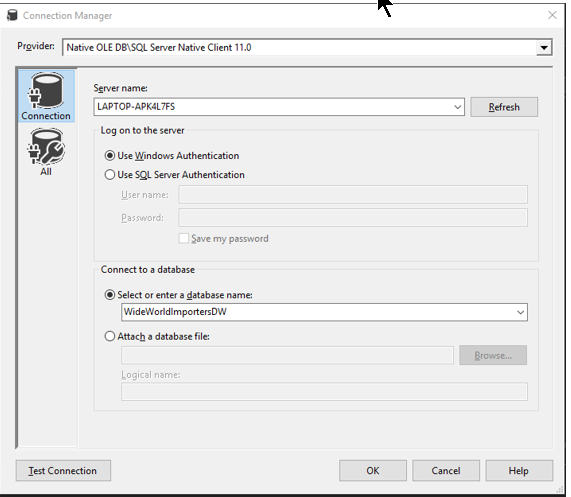
\includegraphics[width=17cm]{IMG/31.png} 
\end{center}

Luego escogemos la base de datos creada de nuestro DataWarehouse\\
\begin{center}
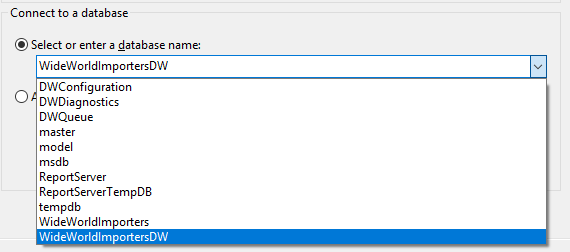
\includegraphics[width=17cm]{IMG/32.png} 
\end{center}

D.	DESARROLLO DE DTSX (DATAFLOW, QUERIES)\\
Esta es la creaci\'on de nuestro Control Flow, en si con sus dimensiones respectivas para cada hecho, que tenemos que es Fact-Sale, Fact-Purchase\\

\begin{center}
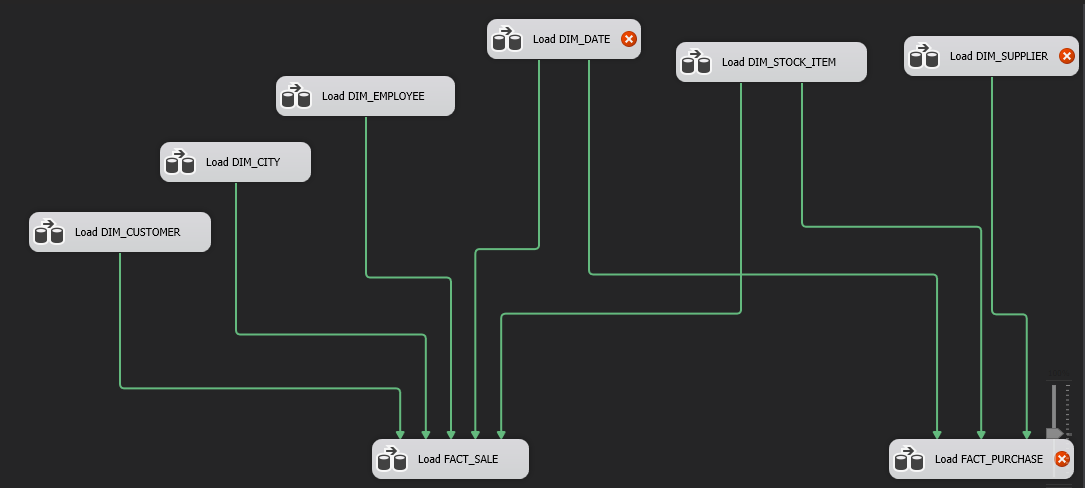
\includegraphics[width=17cm]{IMG/33.png} 
\end{center}

Ahora vamos a crear el Data Flow para cada uno de nuestras dimensiones y luego tambi\'en para los hechos\\
\begin{center}
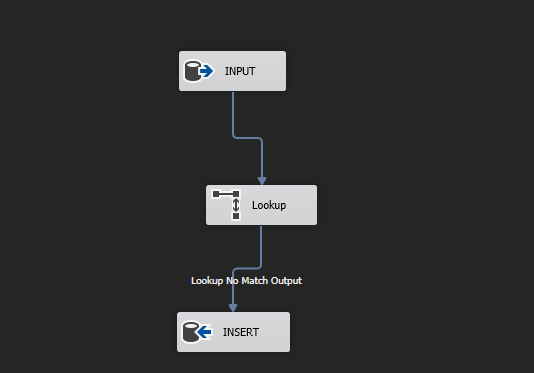
\includegraphics[width=17cm]{IMG/34.png} 
\end{center}

Ahora vamos a darle clic en el input, esto es donde vamos a poner nuestra query para llamar los datos pero primero tenemos que poner la conexi\'on de nuestra base de datos transaccional\\
\begin{center}
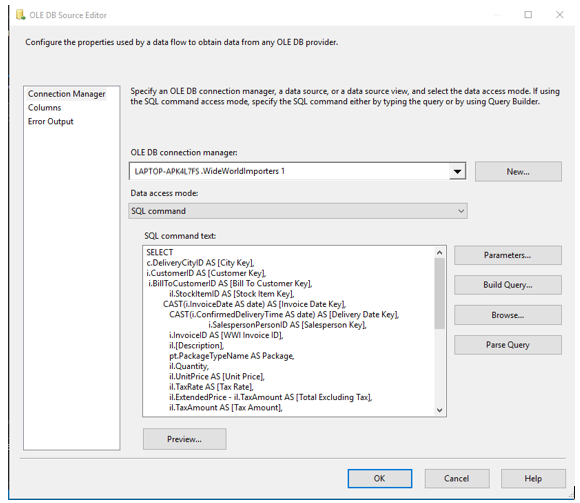
\includegraphics[width=17cm]{IMG/35-m.png} 
\end{center}

Ahora vamos a columnas y vemos que nos jalo todo los datos que hemos puesto, ahora vamos, y luego vamos a dar clic en ok\\
\begin{center}
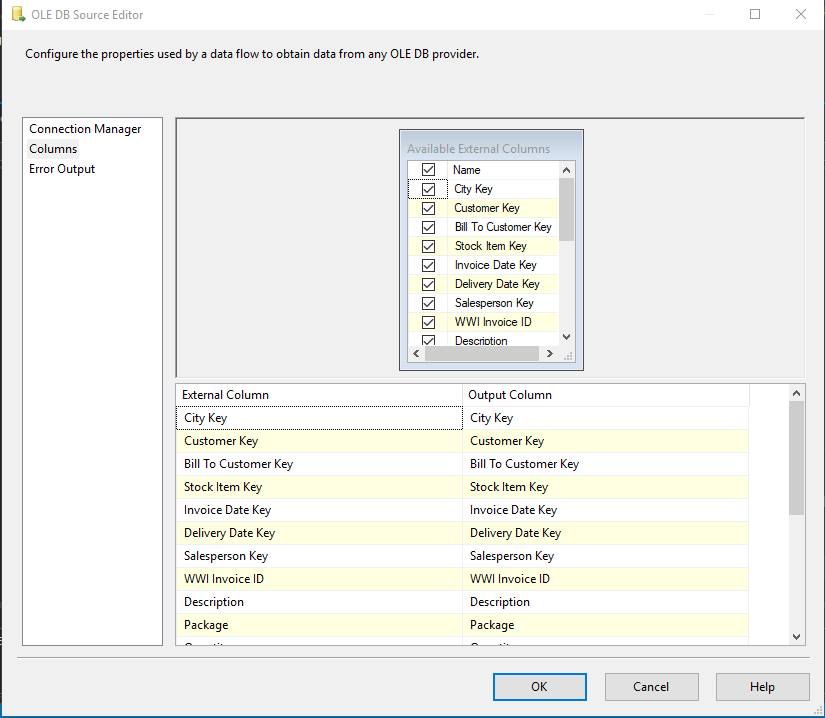
\includegraphics[width=17cm]{IMG/36.png} 
\end{center}

Luego ponemos en general, y ponemos abajo para acabar y luego ponemos en redirect row to no match output, ponemos para que te lo redireccione\\
\begin{center}
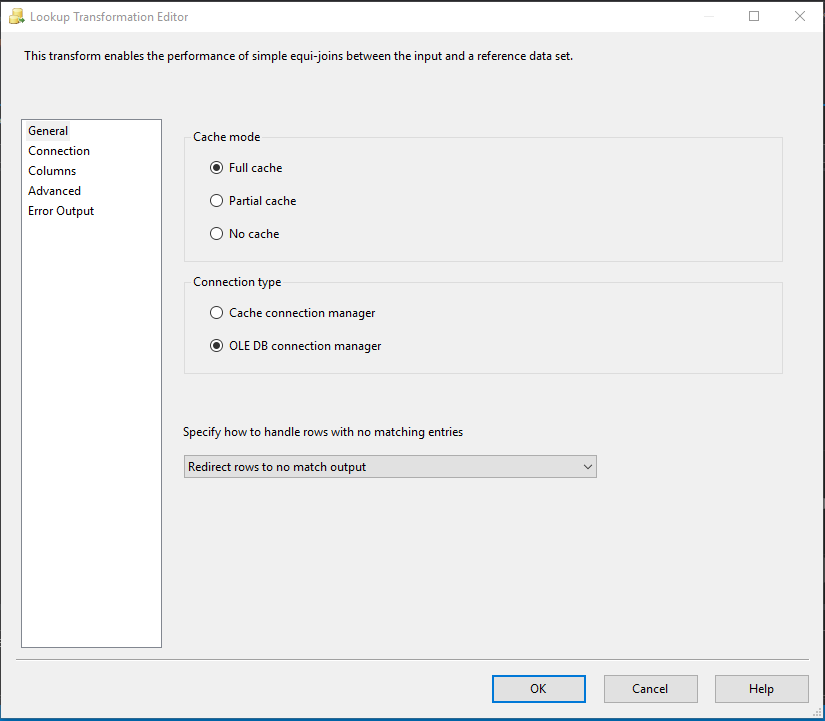
\includegraphics[width=17cm]{IMG/37.png} 
\end{center}

Luego ahora ponemos la conexi\'on que ser\'ia DataWarehouse, y luego seleccionamos la tabla que estamos conectando y luego esta tabla tiene que estar vacía sin datos para que te lo pueda extraer los datos, en el insert\\

\begin{center}
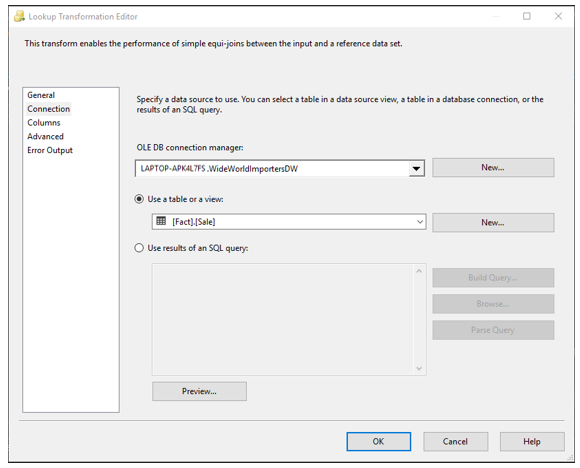
\includegraphics[width=17cm]{IMG/36-m.png} 
\end{center}

Luego ponemos en columnas y como vemos se relaciona normal\\
\begin{center}
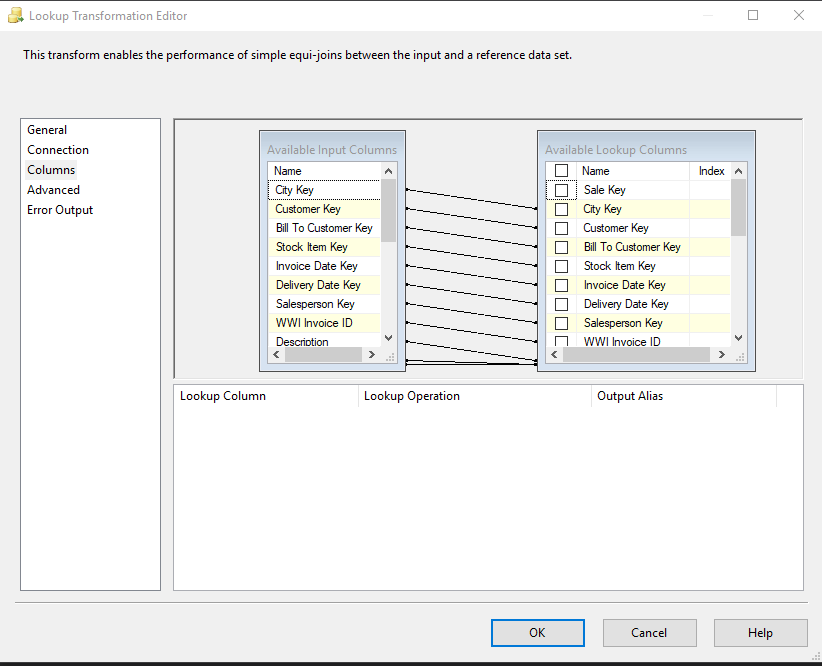
\includegraphics[width=17cm]{IMG/38.png} 
\end{center}

Luego ponemos la base de datos del DataWarehouse, luego escogemos la tabla de hecho Fact Sale\\

\begin{center}
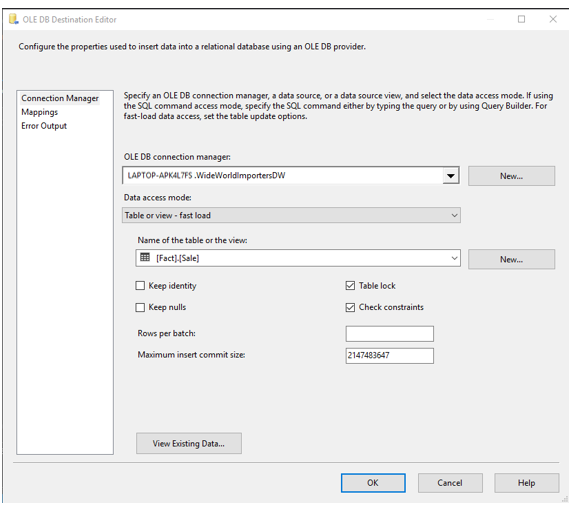
\includegraphics[width=17cm]{IMG/37-m.png} 
\end{center}
Luego ponemos en extracci\'on de datos y como vemos nos jalo todo los datos y luego ponemos clic en close para que lo cierre\\
\begin{center}
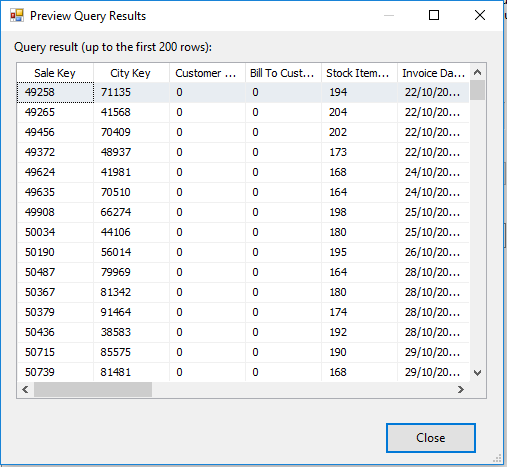
\includegraphics[width=17cm]{IMG/39.png} 
\end{center}
Luego ponemos en mappings, y como vemos se relaciona solamente con cada tabla que ponemos, y le damos clic en ok\\

\begin{center}
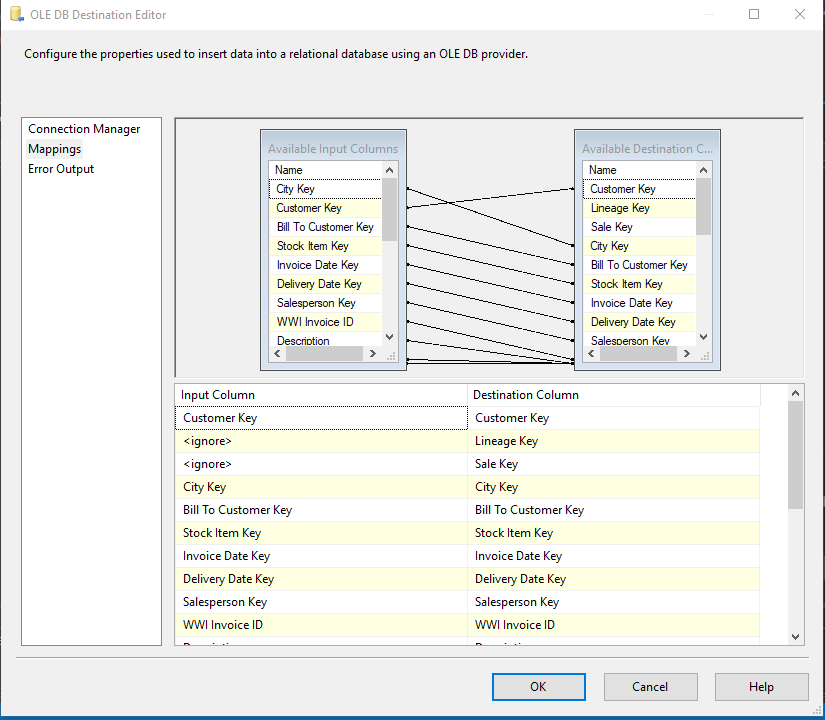
\includegraphics[width=17cm]{IMG/40.png} 
\end{center}
\section{Conclusiones} 

-	Como conclusi\'on hemos visto como realizar una data warehouse y ETL para nuestro proyecto ya que viendo que es importante que primero realicemos nuestra data warehouse para luego poder seguir con nuestro ETL que nos va permitir mover los datos a m\'ultiples fuentes.


\end{document}

